\chapter{Image-based steganography}

In this chapter we will cover the term steganography, explain 
how can we measure its strength. Then we will proceed to image-based
steganography, specifically to JPEG-based one. We will end this chapter
with overview of present state in free and/or open-source software for steganography
(for Android platform).

\section{What steganography is?}

Steganography is an art of hiding information. The difference between steganography and
cryptography is that the goal of cryptography is to hide the content of message, whereas
the goal of steganography is to conceal the very fact that the message exists.

\paragraph{A bit of terminology}

Information, which we want to hide, is often called \textit{secret message}. The object,
in which we want to embed our secret message, is often called \textit{cover message}\footnote{or, in our case,
\textit{cover image}}. Additional information, required to detect and extract the secret message
from cover object, is called \textit{stegokey} (as opposed to cryptokey, which is used to 
unveil the content of the message). If the stegokey, needed to embed a message is different
from the key, needed to extract it, we call this steganographic method \textit{asymmetric}. In
other case, we call it \textit{symmetric}.

\section{How to measure strength of steganographic methods?}

Basic idea is simple: if a message concealed by method X was not discovered, then it's a good method.
But the concealing power depends on the message length (example: it is relatively easy
to write one date on your schooldesk without having your professor seeing it, but it's a lot
harder to write a whole textbook on it). 

Keeping that in mind, one can never tell with $100\%$
guarantee that this object doesn't carry any message, as sometimes it could carry only one bit 
(e.g. wearing the hat; having newspaper in your left hand; sending a postcard; etc.).

So instead another method is often used: whether the attacker can predict (or rather guess) the
length of embedded message.

\section{Image-based steganography}

How to hide messages in lossless image formats and why it isn't a good idea.

\section{JPEG compression algorithm}

JPEG format provides many options for storing images. We will talk about
one of the most common versions. %For further details we recommend to read \TODO source.

Input of compression algorithm is a raw image with pixels encoded
in RGB model (each pixel is encoded as three 8-bit numbers, representing
red, green and blue component of resulting colour, resluting in 24 bits of information
per pixel).

Compression consists of several steps:
\begin{enumerate}
    \item Transformation from RGB to YCbCr color space
    \item Reduction of Cb and Cr channels definition (lossy operation)
    \item Splitting each channel into $8 \times 8$ bytes long blocks 
    \item Discrete cosine transformation (DCT) of numbers in each block
    \item Rounding of DCT coefficients (main lossy operation)
    \item (Lossless) compression of coefficients (main compression operation)
\end{enumerate}

\subsection{Color space transformation}

Pixels are transformed from RGB to YCbCr color space. Y channel represents
brightness of a pixel\footnote{which can be viewed as greyscale copy of the original image},
Cb and Cr components represent so called \textit{chrominance} -- color without brightness. 
You can see example in figure \ref{img:YCbCr}.


%(based on source: \url{https://en.wikipedia.org/wiki/File:Barns_grand_tetons_YCbCr_separation.jpg})
\begin{figure}
%vlozenie samotneho obrazku vycentrovaneho a vhodnej velkosti
%obrazok je v subore images/cervik.png
\centerline{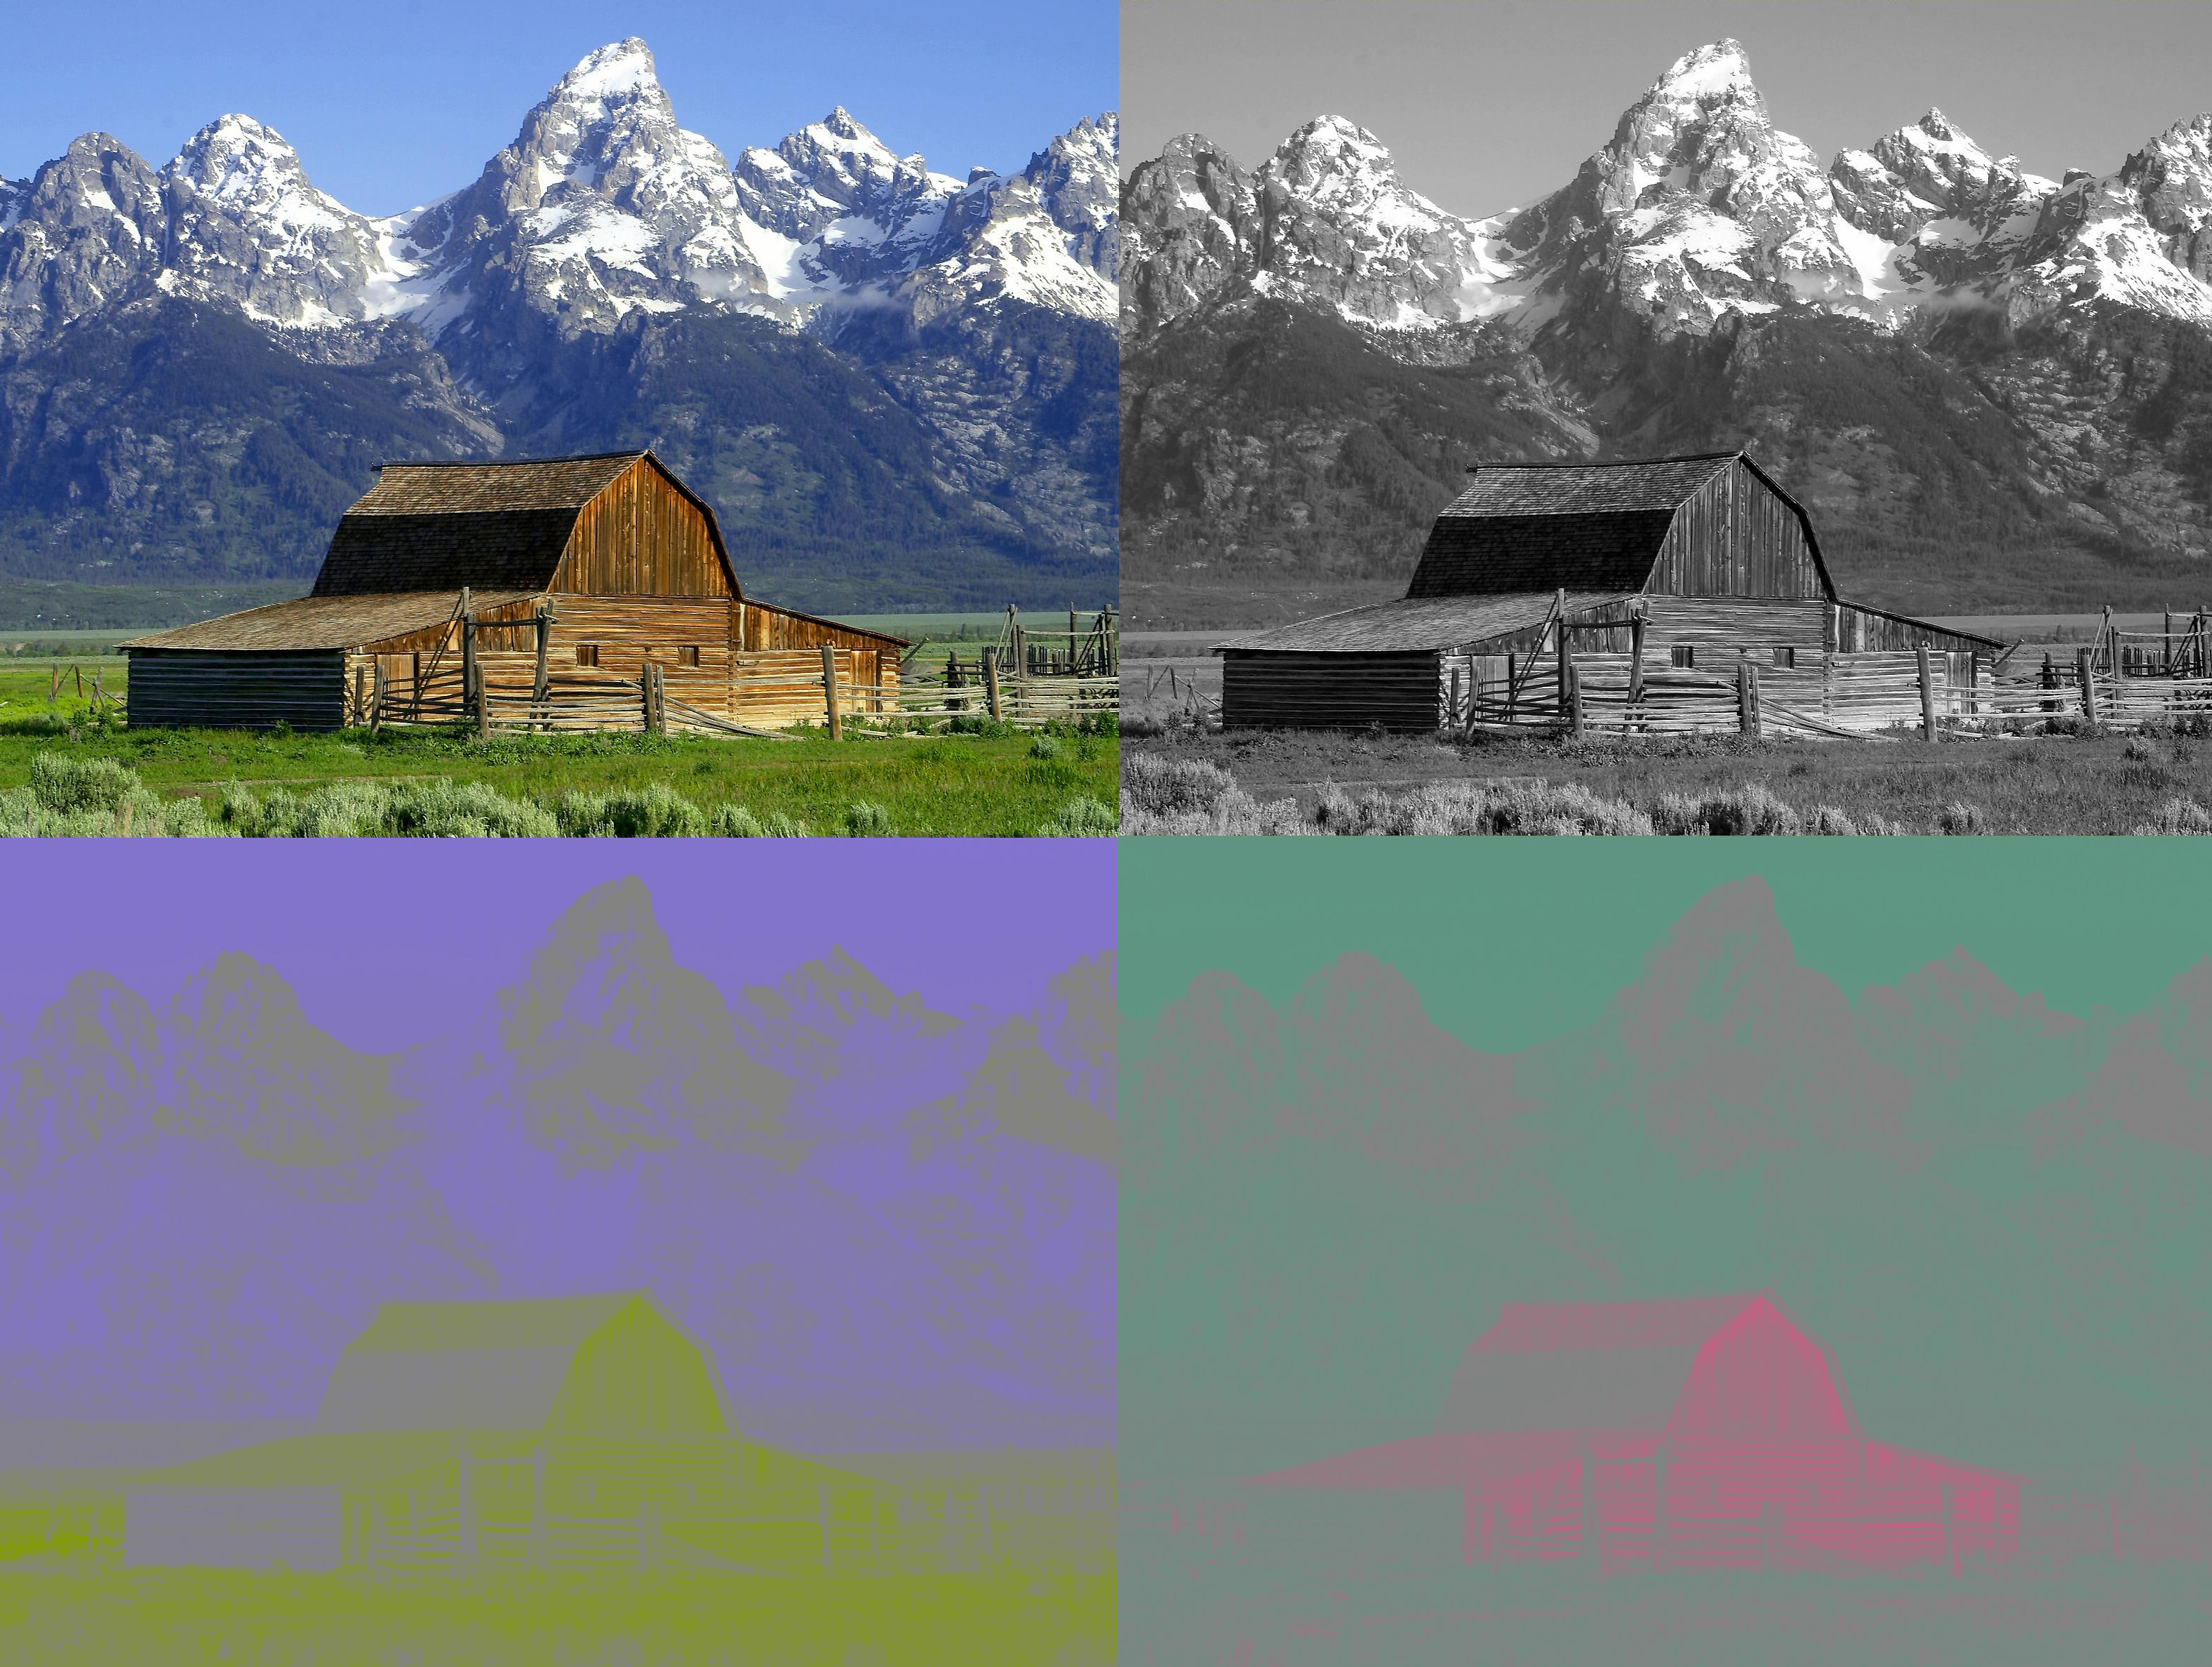
\includegraphics[height=0.4\textheight]{images/Barns_grand_tetons_YCbCr_separation_quad.jpg}}
%popis obrazku
\caption[Example of YCbCr color space (Public domain)]{Example of YCbCr color space. 
Left upper corner is an original image,
right upper corner --- Y channel (grayscale version of image),
left lower --- Cb channel,
right lower --- Cr channel.}
%id obrazku, pomocou ktoreho sa budeme na obrazok odvolavat
\label{img:YCbCr}
\end{figure}

\subsection{Downsampling}

Human eye is more sensitive to small changes of brightness rather 
than small changes in the hue and color saturation. Using that fact, 
we can use less space to represent Cr and Cb channels with almost no visible change
to an image. 

There are many options, but one of the most used is to use 4 bits instead of 8
to represent Cr and Cb and 8 bits to represent Y channel (so Y channel is left unchanged).

\subsection{Splitting into blocks}

Each channel is divided into $8 \times 8$ bytes long blocks and 
then processed separately. If channel is not exact multiple of block size,
then incomplete blocks are filled with fake values (there are several
methods to construct them, but details are irrelevant for our purposes. 
%For further information, you may read \TODO source
).

\subsection{Discrete cosine transformation}

\begin{comment}
Each block could be seen as finite integer sequence.
This sequence can be seen as values of some function $f$ 
in predefined points $x_1$, $x_2$, \ldots, $x_{64}$.

Discrete cosine transformation is a way of representing this
function as a linear combination of sinusoids (so called \textit{basis functions}) 
based on values of $f(x_1)$, $f(x_2)$, \ldots, $f(x_{64})$. Coefficients of this
linear combinations are called \textit{the DCT coefficients} and
are stored instead of original values, because the original 
values can be later evaluated from them. Figure \ref{img:DCTbf} shows the basis functions.

\end{comment}

Dicsrete cosine transformation is a way of representing block of pixels as 
a linear combination of so called \textit{basis functions}, showed on figure \ref{img:DCTbf},
so we can store coefficients of linear combination instead of the original values.

% source: \url{https://en.wikipedia.org/wiki/File:Dctjpeg.png}
\begin{figure}
%vlozenie samotneho obrazku vycentrovaneho a vhodnej velkosti
%obrazok je v subore images/cervik.png
\centerline{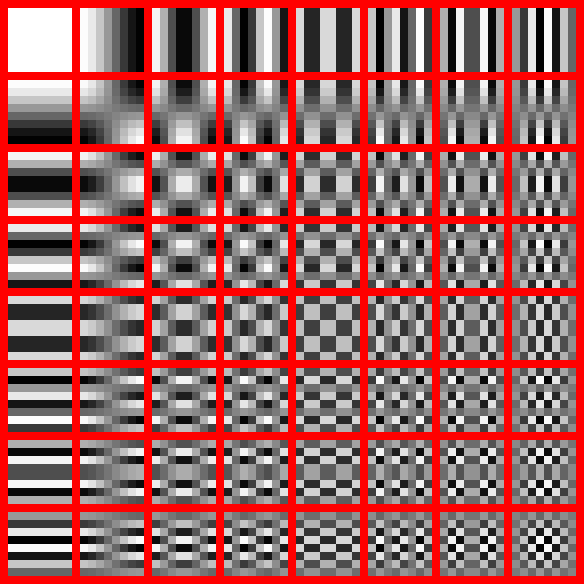
\includegraphics[width=0.5\textwidth]{images/Dctjpeg.png}}
%popis obrazku
\caption[DCT basis functions (Public domain)]{DCT basis functions.}
%id obrazku, pomocou ktoreho sa budeme na obrazok odvolavat
\label{img:DCTbf}
\end{figure}



\subsection{Rounding of DCT coefficients}

Here we use two facts. First, DCT basis functions varies from simple
to very complex. Second, human eye is less capable to distinguish such
fine local changes. Therefore, we can represent coefficients of complex
basis functions with less definition (in other words, quantize them).

The level of quantization is defined by demanded quality ratio.

The most fine quailty $Q=100\%$ let all coefficients be rounded to whole numbers.

\subsection{Lossless compression of DCT coefficients}

Another interesting property of DCT is that the coefficients
of last basis functions are often very small (because DCT "tries"
to express image with the first sinusoids). Therefore, after
quantisation process many of DCT coefficients could be zero.

As could be expected, long sequences of zeros could be efficiently
compressed, and therefore significant compress ratio could be achieved.


\section{How to hide information in JPEG?}

\textit{This section is based on article \cite{liu2008high}.}

An image encoded in JPEG format could be seen as a bunch of (quantized)
DCT coefficients, which are just regular integer numbers. One of the
most natural ideas is to change least significant bits (LSB) of these
numbers to store our message, as these changes are mostly invisible
for human eye and the message can be extracted without knowledge of
the original image.

Problems with direct application of this method is that coefficients with values
$0$ or $1$ would be changed drastically and it would create great disproportion
in amount of zeros and ones.

Modern algorithms tries to fight with statistical approach by devising ways to
keep intact various statistical properties of resulting numbers. 

\subsection{JSteg library (direct LSB)}

This library embed secret message in LSB of DCT ceofficients sequentially,
but it skips coefficients which are equal to $0$ or $1$. This way the amount
of 0s and 1s is kept intact.

But this approach is really unsecure as it can be easily detected by so called
\textit{chi-square attack}.

\subsection{Chi-square attack}

Assuming that 0 and 1 bits are distributed uniformly in the secret message 
(which is usually the case for compressed and/or encrypted message), relative
amount of values, which differ only in their LSB (so called \textit{paired values}),
becomes equal. And assuming sequential writing in DCT coefficients, one can test
whether paired values show such behaviour. The corresponding statistics has chi-square
distribution, from which this attack got its name.

This attack could be extended to random writing (i.e. that DCT coeficients to write next bit
are chosen randomly), so we can speak about \textit{extended chi-square attack}.

\subsection{F5 algorithm}

In order to defend against chi-square attack, Westfield and Pfitzmann proposed F5 algorithm.
Instead of replacing LSB to match secret message, it decreased the absolute values of randomly 
(using stegokey) chosen DCT coefficients (skipping 0s and 1s), so it won't be detected by
chi-square attack.

This approach can be broken using S family attack.

\subsection{S family attack}

This attack is based on further compression of cover image ans comparing 
specifically constructed statistics $S$ of the original and compressed images.

% Details can be read here \TODO source.

\subsection{Complementary embedding algorithm (Liu and Liao)}

This algorithms is designed to fight with both S and chi-square attacks families.

It divides secret message into 2 parts, and embed it at randomlychosen DCT coefficients,
but for first part, it encodes bits by adding one to DCT coefficient if the value of 
secret bit is 1, and for the second part, it subtract 1 instead. Therefore, as the article
\cite{liu2008high} shows, it can successfully pass through both of these tests.

\subsection{Bernford law}

\section{Present state of free and/or open-source programs}
